\chapter{Resultados}
\label{ch:chap4}

En esta sección se presentan varios resultados y la mayoría pueden explorarse de manera casi independiente uno de otro. Sin embargo, todos los resultados presentados en la tesis, salvo los resultados presentados en la sección~\ref{sec:sec41}, están reducidos a las 40,000 palabras de uso más frecuente con base en el CREA.

\section{Corpus}
\label{sec:sec41}

\section{Análisis de las proyecciones}
El \textit{embedding} de palabras es la representación de $N$ palabras en un subespacio de $\mathbb{R}^K$ de dimensión entre 100 y 600. Bajo la métrica coseno, por ejemplo, la palabra \textit{madre} está altamente relacionada\footnote{En este ejemplo, se empleó un corte arbitrario de 0.75 para determinar esto. En la literatura no autor que especifique donde se debe hacer el corte para recuperar las palabras ``similares''.} con la palabras: \textit{padre}, \textit{hija}, \textit{mamá}, \textit{hermana} y \textit{abuela}. 

El ejemplo es un excelente ejemplo de como la métrica coseno recupera relacionadas. Pero es necesario hacer notar que la métrica no establece una relación de orden adecuada. Mayor cercanía debería traducirse en mayor parecido en significado. Pero, en el ejemplo mencionado se tiene que la distancia de \textit{madre} con \textit{padre} fue de 0.76, de \textit{madre} con \textit{hija} fue de 0.81, de \textit{madre} con \textit{mamá} fue de 0.78, de \textit{madre} con \textit{hermana} fue de 0.77 y, de \textit{madre} con \textit{abuela} de 0.75. Por lo tanto, la palabra \textit{hija} está más relacionada con la palabra \textit{madre} \textit{madre} que la palabra \textit{mamá}.

Otro detalle particular radica en determinar un criterio para determinar ``alta'' similaridad. Al relajar el criterio de similaridad la palabra \textit{madre} se encuentra relacionada con varias palabras como \textit{mujer}, \textit{familia}, \textit{marido}, \textit{nuera}, \textit{tía}. Palabras que con claridad tienen una relación con la palabra \textit{madre}. Esto permite establecer un campo semántico donde existen todo tipo de relaciones: Meronomia, donde por ejemplo, \textit{madre} e \textit{hija} forman parte de \textit{familia}; Sinonimia en la relación de \textit{madre} con \textit{mamá}; Hiponimia en la relación \textit{abuela} y \textit{madre} y; Lineales en la relación \textit{madre} e \textit{hija}.

Sin embargo, bajo ese mismo umbral de similaridad, la palabra \textit{vida} resulta similar a \textit{cotidiana}. Lo cual da sentido pues ``vida cotidiana'' es un compuesto común; pero no rescata la misma información que se rescata de la palabra \textit{madre} pues \textit{cotidiana} no forma parte del campo semántico de \textit{vida} por si misma; aunque \textit{vida cotidiana} sí podría considerarse parte del campo semántico de \textit{vida}\footnote{Los ejemplos mencionados son producto de un análisis exhaustivo de la información contenida \texttt{distance\_angle.np} y requiere al menos 13 GB de RAM dispoible para su carga completa.}.

Entonces que significan las p

\section{Propuestas en pre-procesamiento del español}


\section{Análisis de métricas}

La metodología descrita en el capítulo~\ref{ch:chap3} permite obtener 

\section{Aplicaciones}

Dentro del PLN existen tareas que podrían llamarse nucleares como lo es la modelación del lenguaje, el cual es el tema principal de este trabajo, y tareas que podrían llamarse como finales o aplicaciones que son la parte visible del PLN. De acuerdo con \cite{srinivasa2018natural} dentro de estas aplicaciones están los asistentes virtuales, las herramientas de atención al cliente como los chatbots, el análisis de sentimiento y la clasificación de documentos. En esta última parte de los resultados se presentan algunas aplicaciones desarrolladas soportadas en parte de los resultados obtenidos previamente mencionados: Bot Agricultor, Analizador de Opiniones de Foros Educativos y Facebook Miner\footnote{Cada una de las aplicaciones surgió de las pláticas con otras personas que me contaron una idea y que en su momento me pareció una buena para poner a prueba parte de los resultados obtenidos en este trabajo.}. 

\subsection{Bot Agricultor}

A través del Sistema Nacional del Información e Integración de Mercados (SNIIM) la Secretaría de Economía proporciona información histórica sobre tres mercados importantes en el país: agrícola, pecuario y pesquero. En 2018 Detags y la Universidad Autónoma de Querétaro acercaron la información del mercado agrícola al pequeño y mediano agricultor con un resultado favorable por medio de una plataforma de Shiny R y de la experiencia obtenida surgieron dos peticiones: precios futuros y consultas sencillas e informativas \citep{detags}. El bot agricultor representa una solución a la petición de consultas sencillas\footnote{A diferencia de código fuente usado a lo largo de este trabajo, el Bot Agricultor se encuentra en el siguiente repositorio: \url{https://github.com/Wilfridovich17/germinando}.}.

El bot agricultor es un chatbot. Un chatbot, de acuerdo con \cite{khan2017build} es un programa que procesa lenguaje natural del usuario y genera una respuesta útil al usuario; aunque en la práctica la mayoría sigue una estructura basada en reglas donde se le va pidiendo al usuario que responda una pregunta con alguna de las opciones válidas mostradas en pantalla para al final dar respuesta a la solicitud (Fig~\ref{fig:chatbots}).

\begin{figure}[h]
	\centering
	\begin{subfigure}{0.45\linewidth}
		\centering
		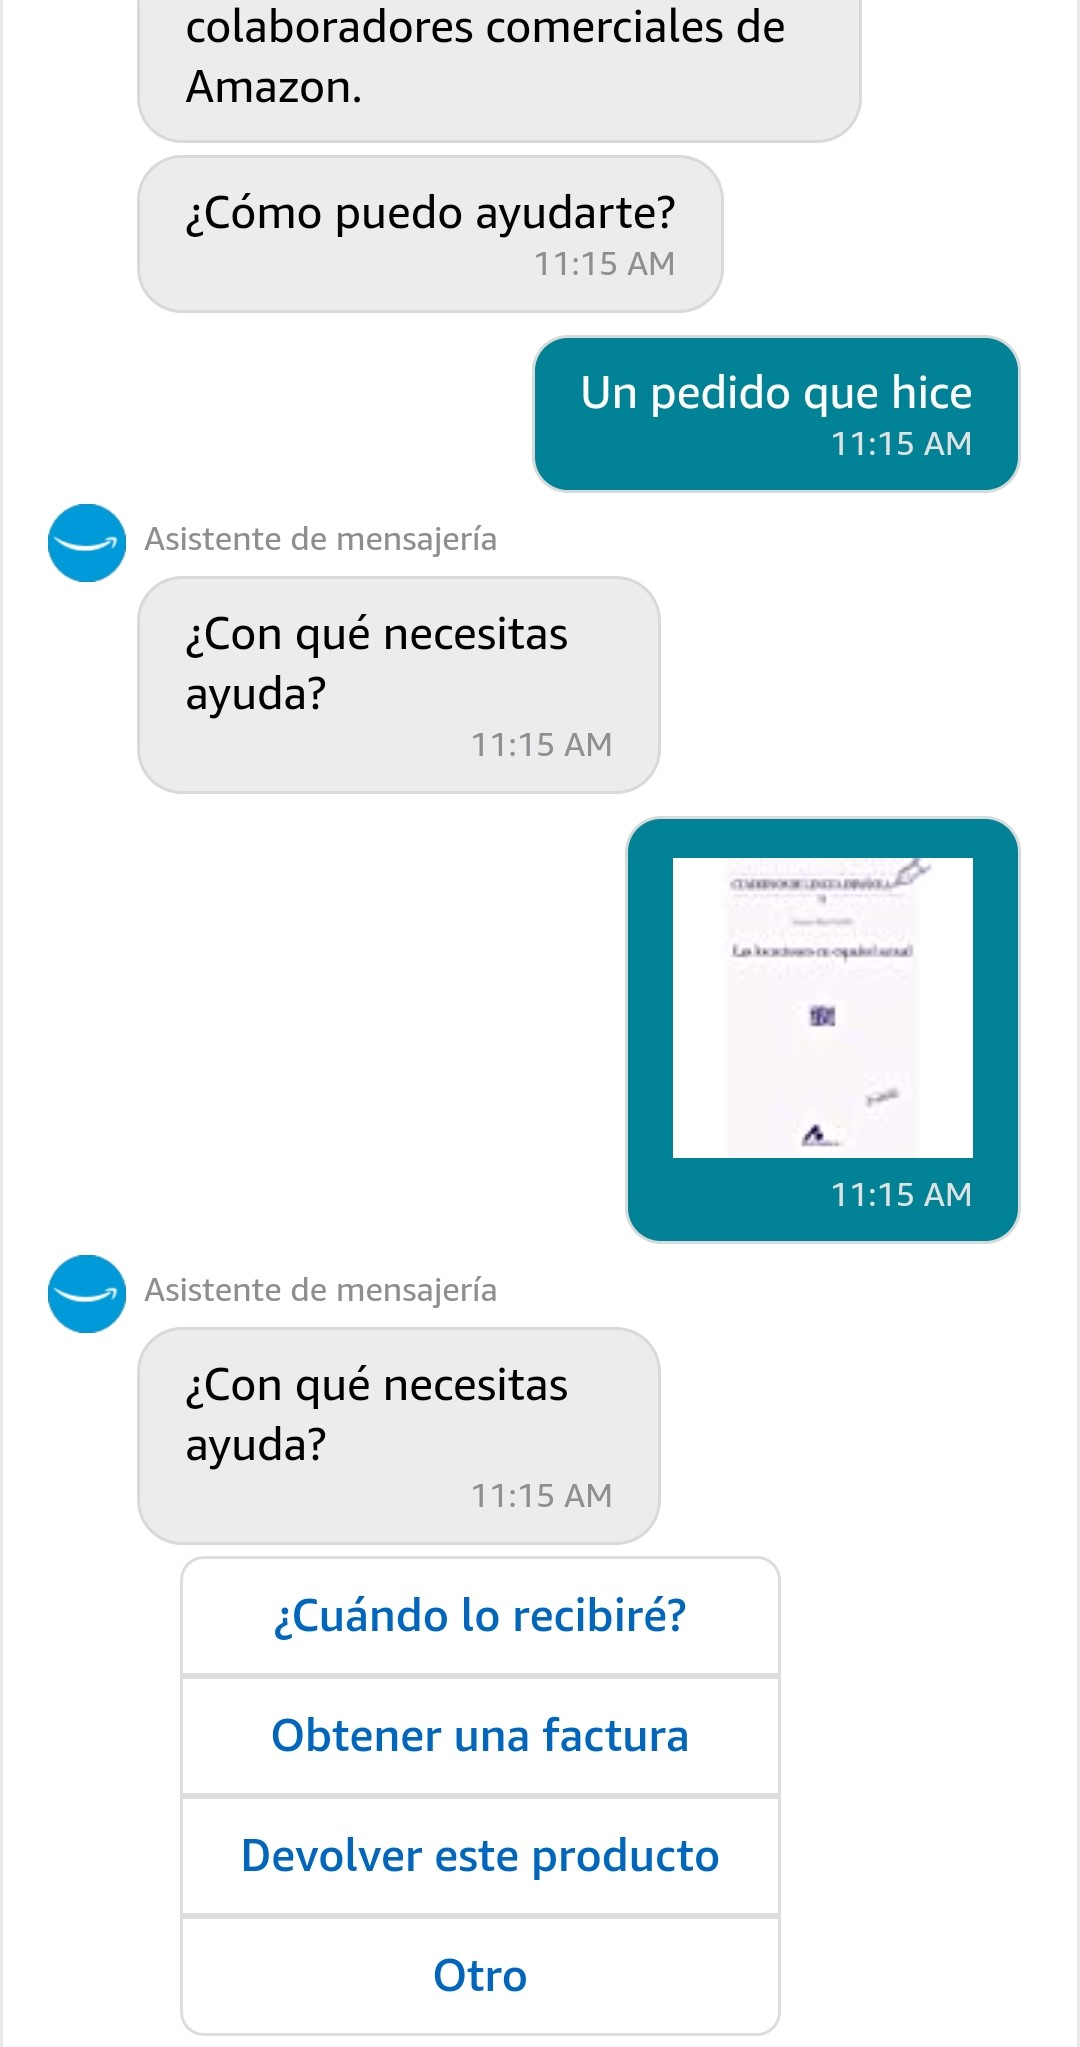
\includegraphics[width=0.45\linewidth]{img/chatbotamazon2}
		\caption{Chatbot de Amazon}
		\label{fig:chatbotamazon}
	\end{subfigure}
	\begin{subfigure}{0.45\linewidth}
		\centering
		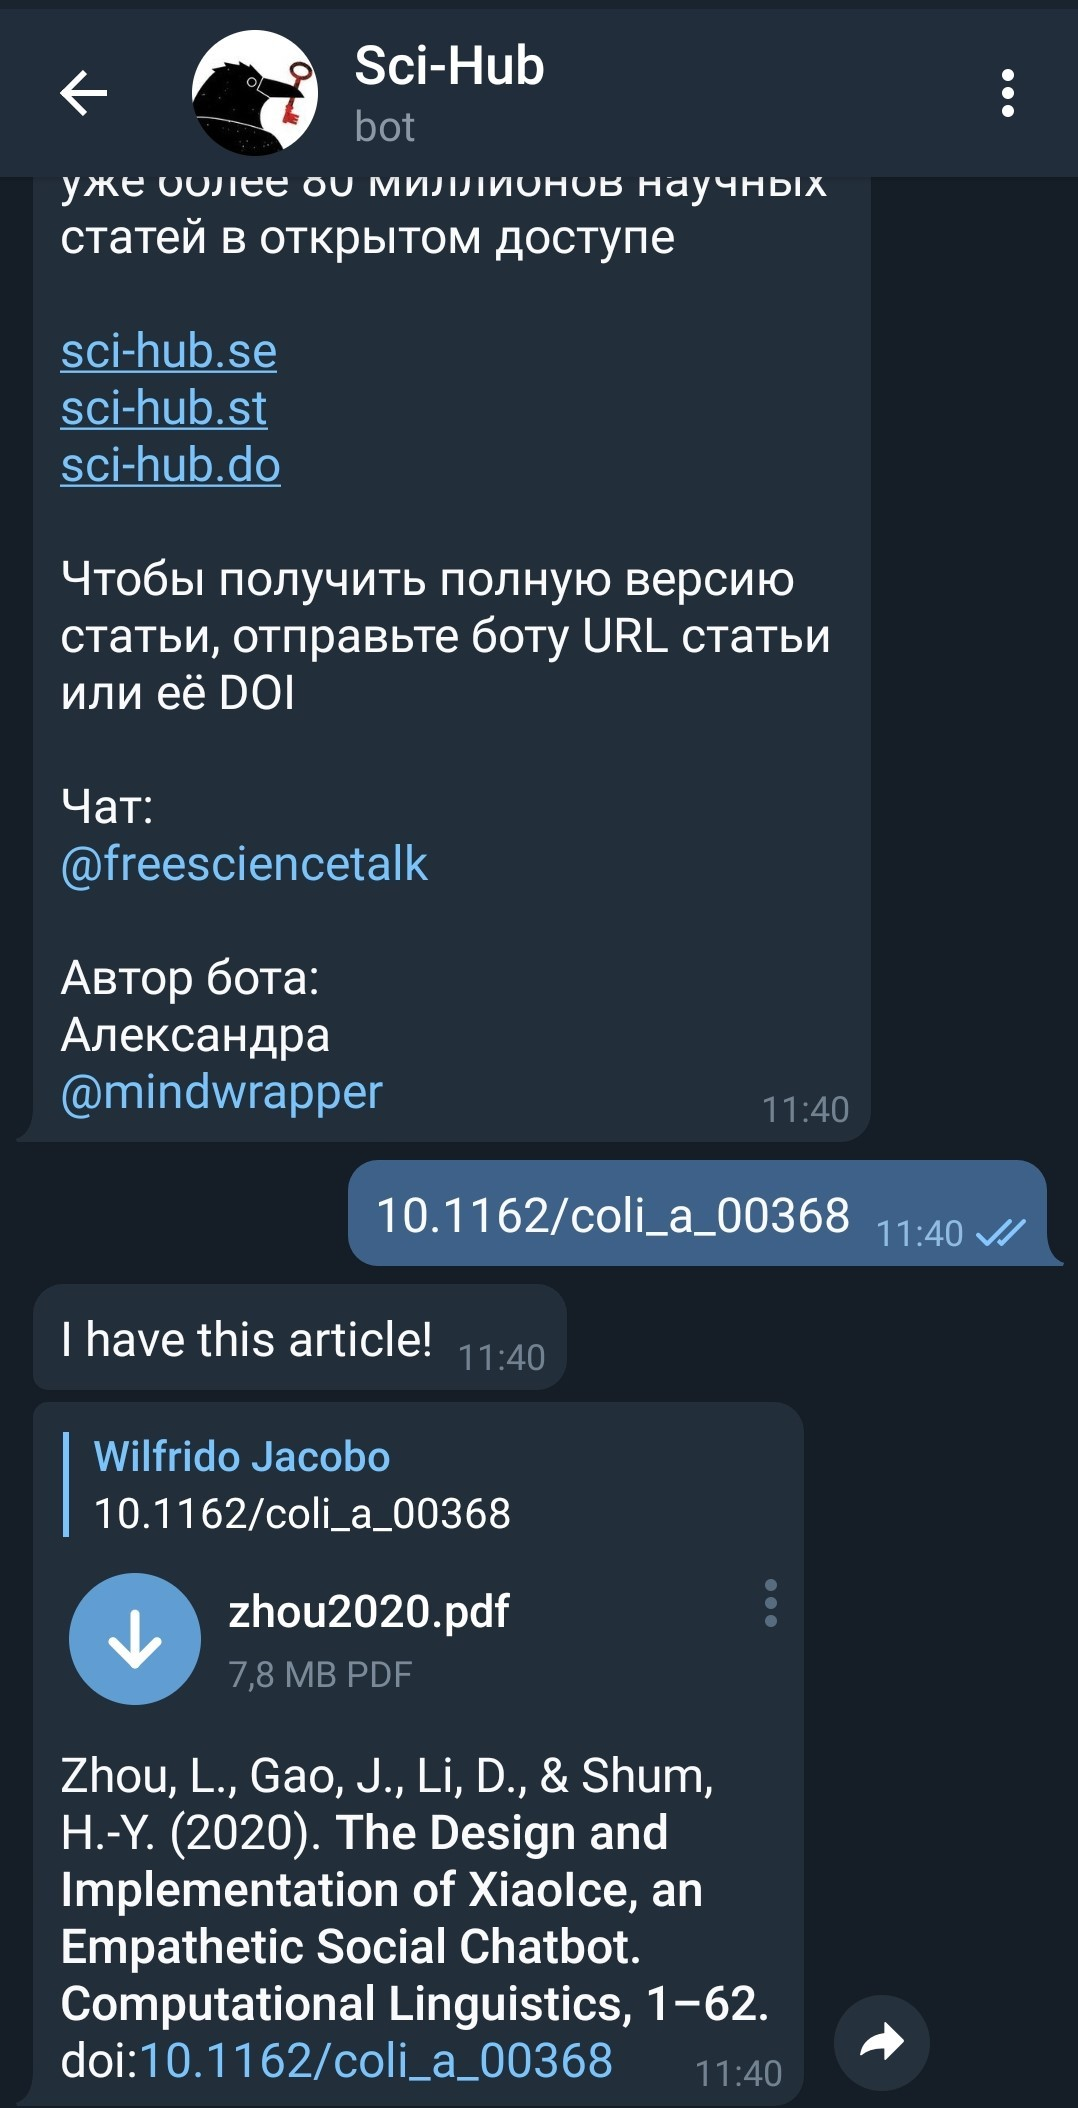
\includegraphics[width=0.45\linewidth]{img/chabotscihub}
		\caption{Chatbot del Sci-Hub}
		\label{fig:chatbotscihub}
	\end{subfigure}
	\begin{subfigure}{0.45\linewidth}
		\centering
		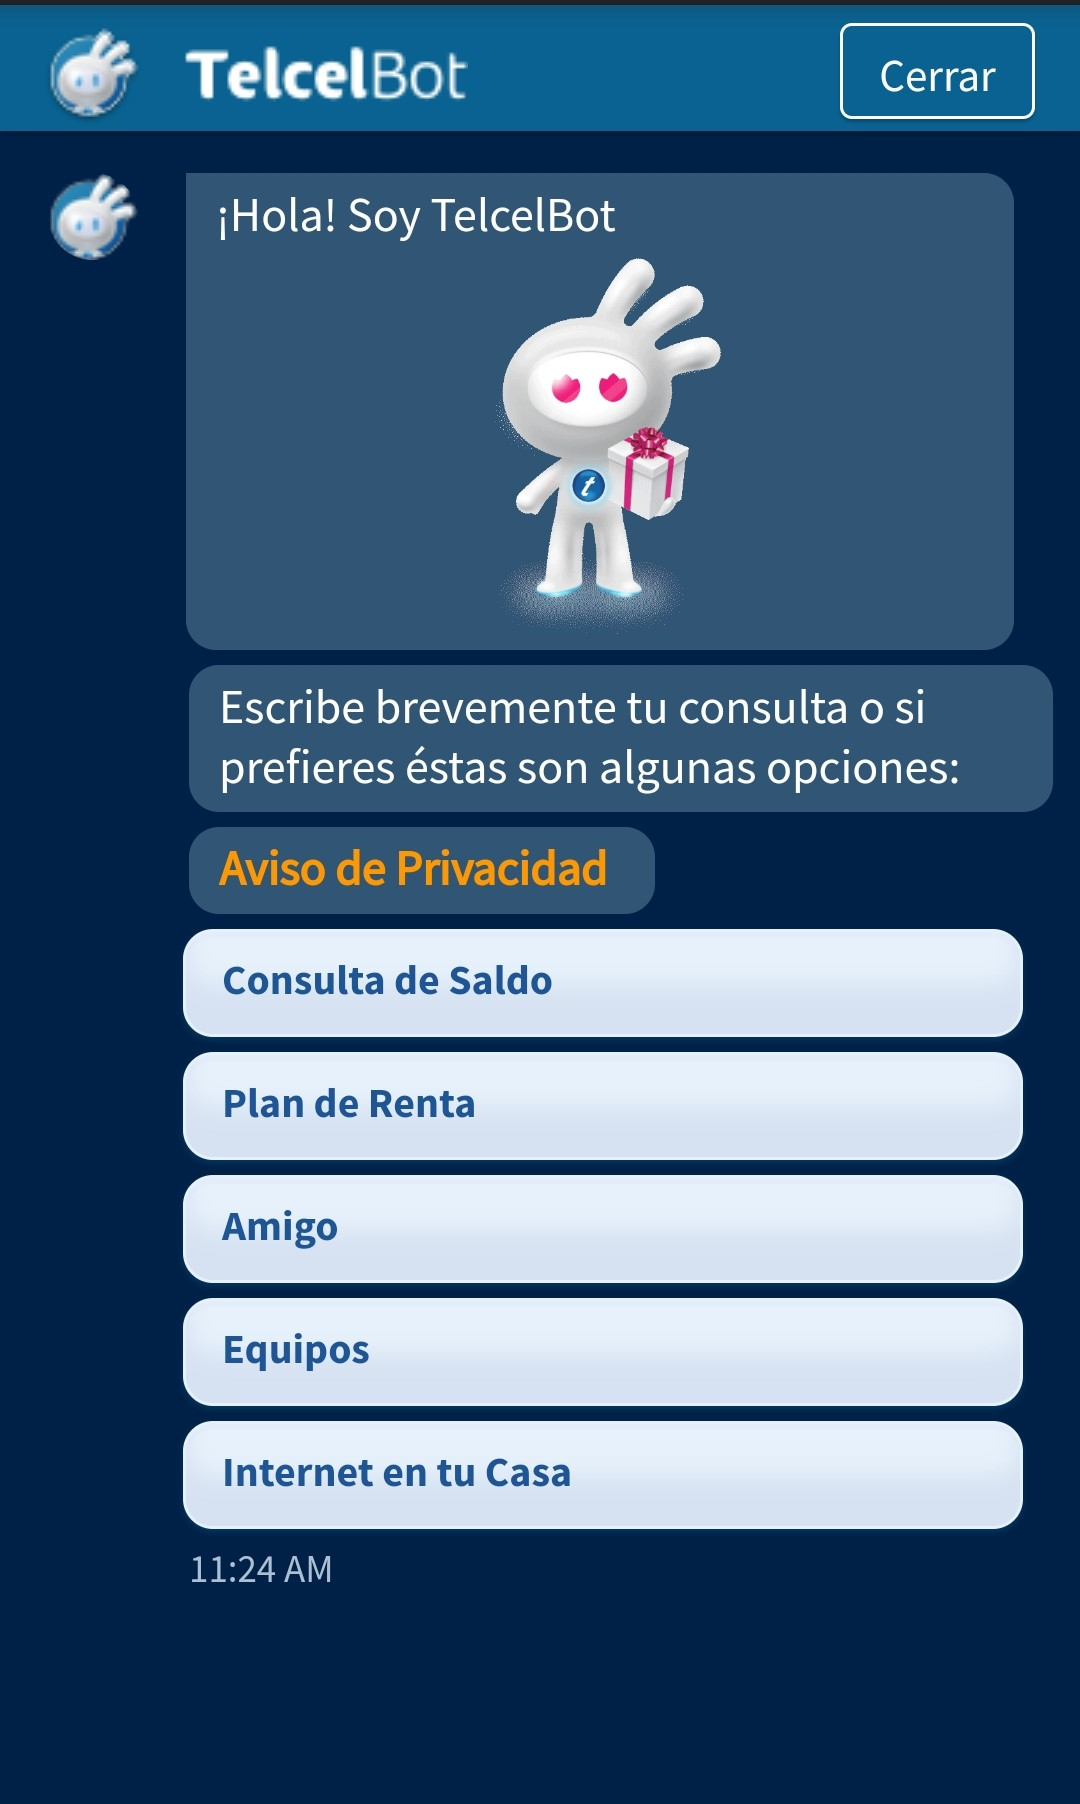
\includegraphics[width=0.45\linewidth]{img/chatbottelcel}
		\caption{Chatbot de Telcel}
		\label{fig:chatbottelcel}
	\end{subfigure}
	\begin{subfigure}{0.45\linewidth}
		\centering
		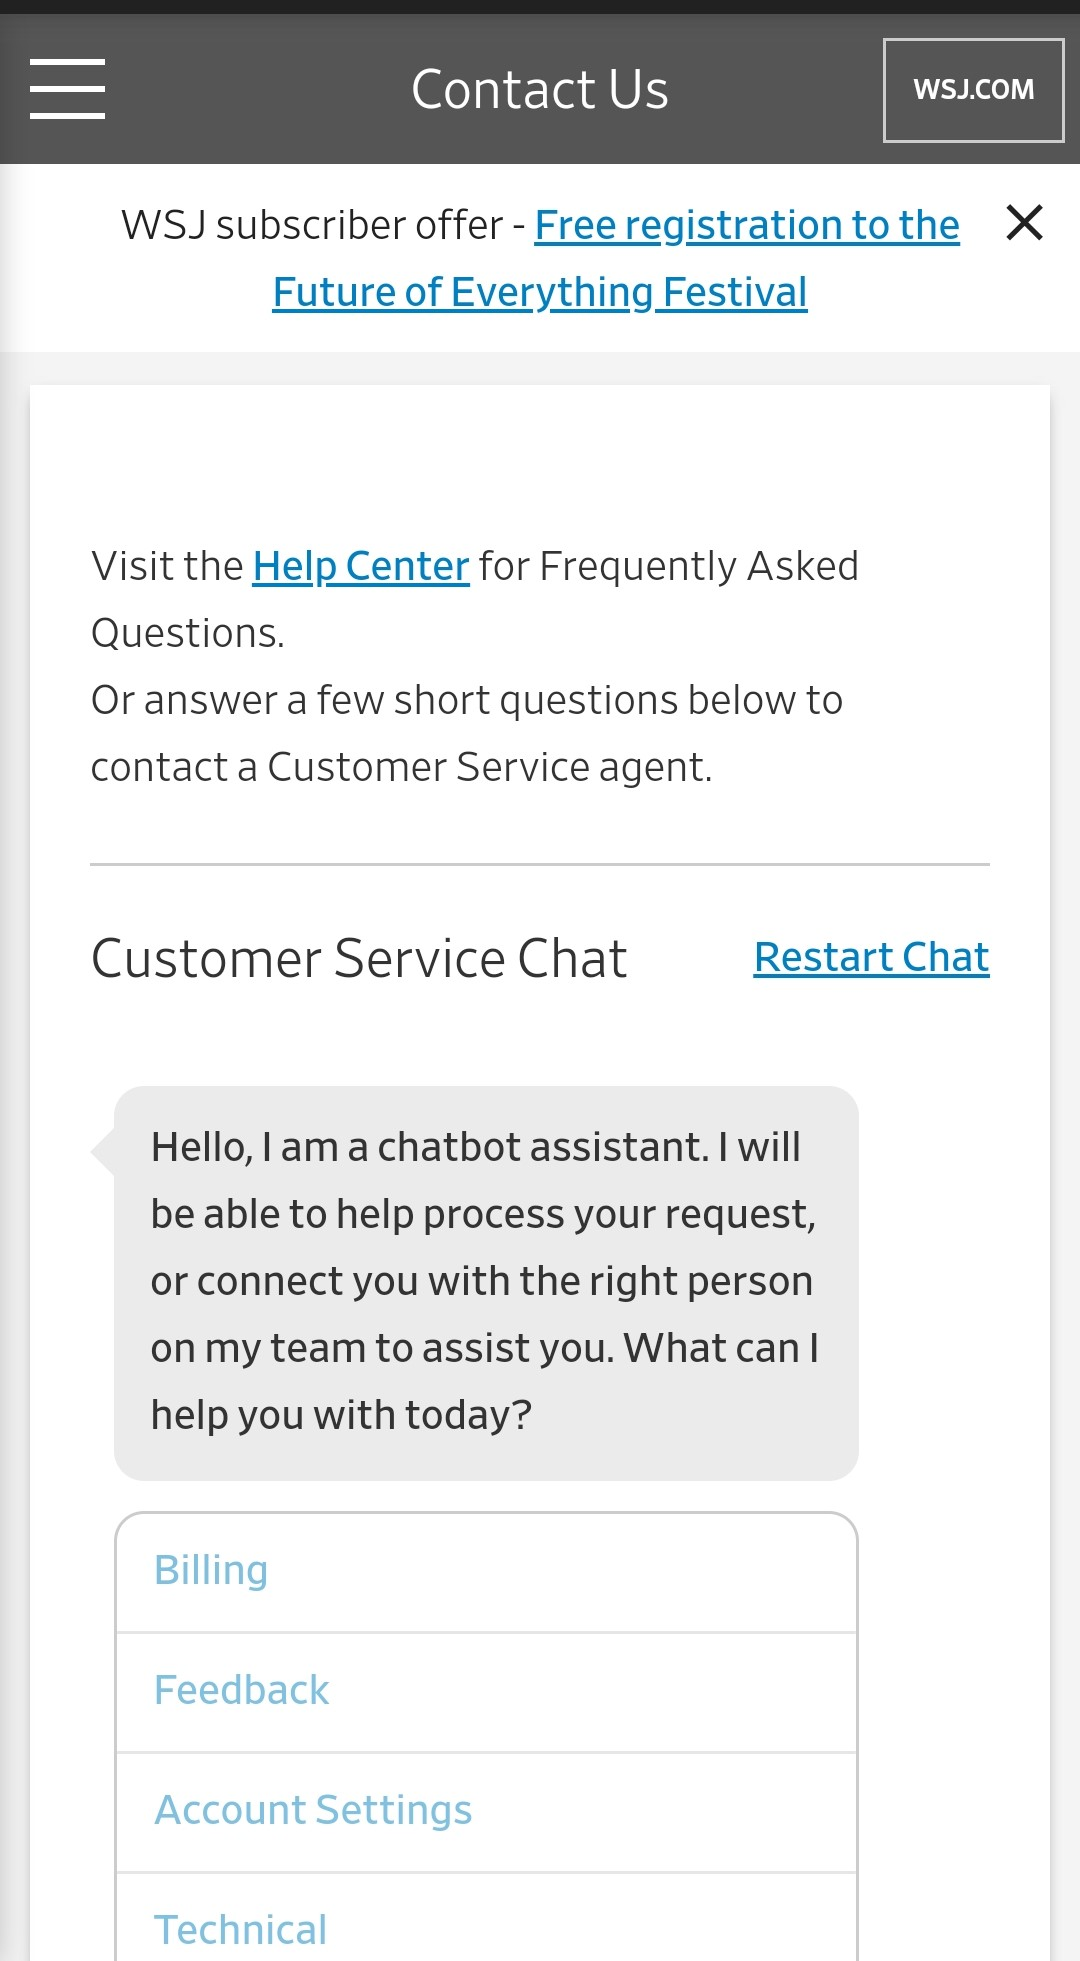
\includegraphics[width=0.45\linewidth]{img/chatbotwsj}
		\caption{Chatbot del Wall Street Journal}
		\label{fig:chatbotwsj}
	\end{subfigure}
	\caption{Ejemplos de chatbots. Obtenidos mediante una captura del pantalla al sitio del proveedor del servicio al interactuar con el chatbot.}
	\label{fig:chatbots}
\end{figure}

En el contexto de las consultas al SNIIM se definieron cuatro tipos de peticiones que fueron clasificadas en: resumen, predicción, precios (históricos) y comparación, las cuales se implementaron en un chatbot de Telegram similar al empleado por Sci-Hub\footnote{Para más información para la creación de un bot en Telegram se puede consultar la siguiente liga \url{https://core.telegram.org/bots}}. Tales peticiones tienen una estructura básica de solicitud:

\begin{itemize}
	\item \texttt{@Resumen Aguacate Hass en Querétaro}
	\item \texttt{@Precio Aguacate Hass en Queretaro 17-04-2020}             
	\item \texttt{@Predice Aguacate Hass en Queretaro 7 días}            
	\item \texttt{@Compara Aguacate Hass en Queretaro 40}
\end{itemize}

Estas instrucciones se traducen de manera sencilla a una \textit{orden} la cual se maneja usando un diccionario de Python. Por ejemplo la instrucción \textit{predice} se codifica como sigue:

\begin{center}
	\texttt{orden = \textbraceleft`instruccion':`resumen', `producto':[[`Aguacate Hass']], `mercado':[[28]], `auxiliares':\textbraceleft`Ventana':7, `Longitud':1\textbraceright\textbraceright}
\end{center}

Las solicitudes con estructura básica fueron creadas para que quien interactúe con el chatbot conozca de antemano qué está pidiendo y qué va a terminar entendiendo el chatbot. Sin embargo, se agregó al chatbot un módulo de lenguaje natural, módulo que le permite transformar instrucciones \textit{más naturales} en la estructura de orden antes mencionada (Fig.~\ref{fig:natbot1}). Mientras que, a nivel usuario, las solicitudes son procesadas como se muestra en la Fig.~\ref{fig:natbot2}.

\begin{figure}[h]
	\centering
	\begin{subfigure}{0.45\linewidth}
		\centering
		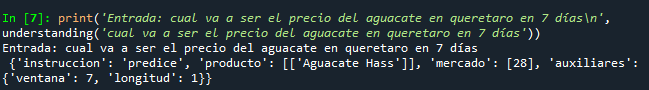
\includegraphics[width=0.9\linewidth]{img/naturalbot1}
		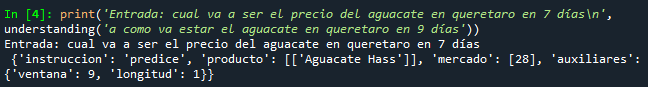
\includegraphics[width=0.9\linewidth]{img/naturalbot2}
		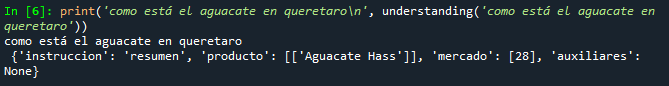
\includegraphics[width=0.9\linewidth]{img/naturalbot3}
		\caption{Ejemplo del funcionamiento del módulo de procesamiento natural del bot agricultor.}
		\label{fig:natbot1}
	\end{subfigure}
	\begin{subfigure}{0.45\linewidth}
		\centering
		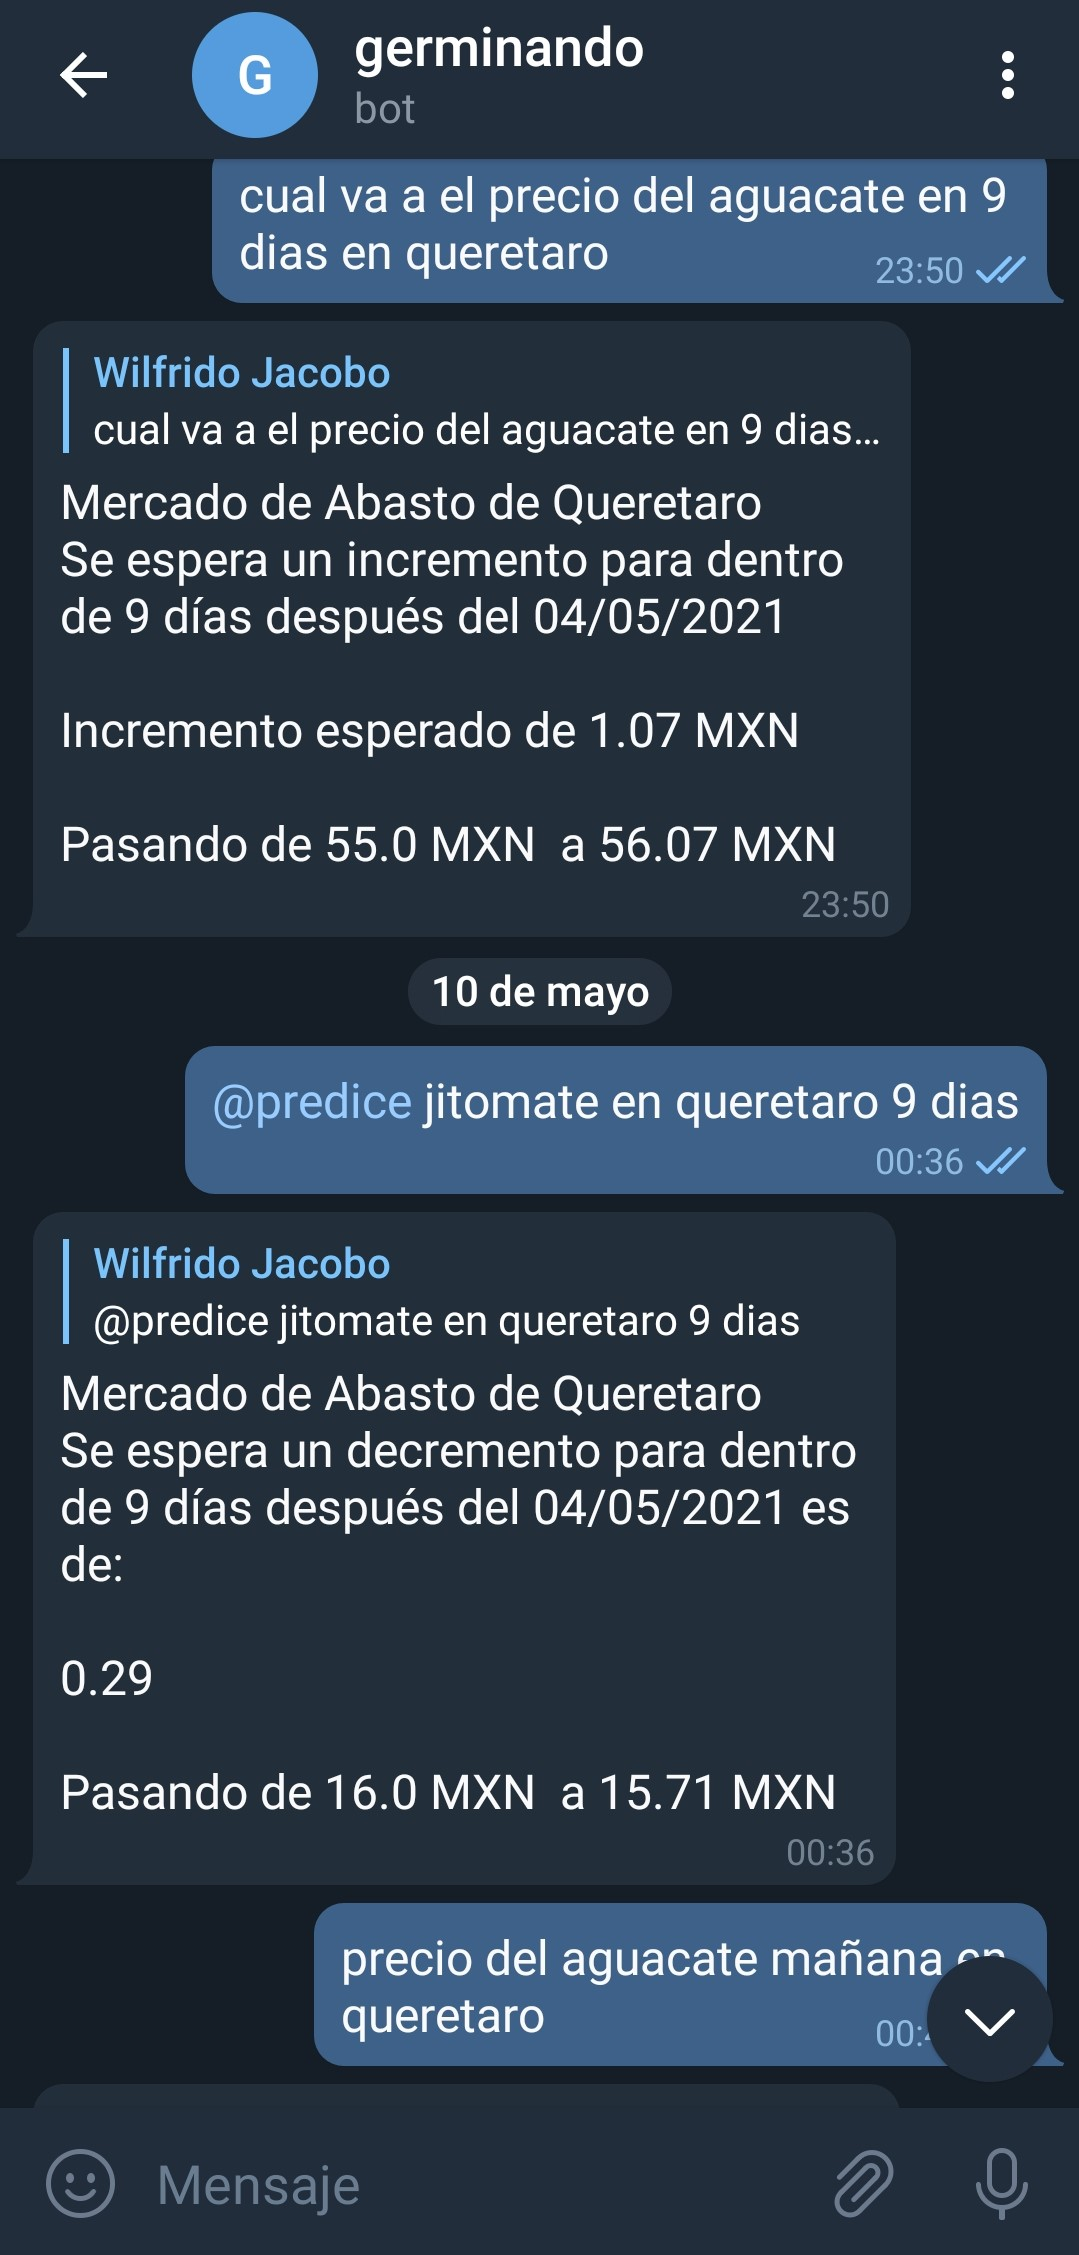
\includegraphics[width=0.45\linewidth]{img/germinandobot}
		\caption{Ejemplo del funcionamiento del bot agricultor a nivel usuario.}
		\label{fig:natbot2}
	\end{subfigure}
	\caption{Bot agricultor donde se muestra la parte trasera del desarrollo y la parte frontal del desarrollo. }
	\label{fig:naturalbot}
\end{figure}


\subsection{Facebook Miner}



\subsection{Análisis de opinión en foros educativos}

De acuerdo con \cite{coviddocentes} para el Banco de Desarrollo Inter-Americano, en la educación a distancia ocasionada por la crisis provocada por el SARS-CoV-2, los profesores sienten que deben estar 24/7 para sus alumnos y dicen sentirse abrumados debido a que reciben una enorme cantidad de llamadas y mensajes fuera de su horario laboral. Además, \cite{teachingcovid} mencionan que la carga laboral de los docentes aumentó drásticamente debido a la generación y adecuación del material para su distribución vía web así como el registro completo de todas las actividades. Sin embargo, el incremento de la carga docente es resultado de las medidas para disminuir la deserción escolar al mantener actividades y contacto con los estudiantes en un horario extendido.

Algunas escuelas dentro de sus medidas para mantener la interacción, han optado por crear foros de discusión para las materias de los estudiantes y fomentar la reflexión e intercambio de ideas entre los estudiantes. Sin embargo, a diferencia del aula tradicional donde la retroalimentación y moderación del docente se realizaba al momento, disponibilidad de los foros impide que los docentes intervengan de manera fluida. En ese sentido, el PLN puede ofrecer una solución parcial mediante una adecuación de un análisis de opinión semántico con el fin de corregir el rumbo de estudiantes que han llegado a una idea que pueda clasificarse de alguna manera como contradictoria.





 

